
 Pour réaliser un tas de sable, Albert creuse un fossé dont les
  parois sont verticales et dont la base est délimitée par deux
  cercles dont l'un a un rayon double de l'autre.\\
  Avec tout le sable extrait il forme au milieu un cône de révolution
  dont la base coïncide parfaitement avec le disque autour duquel il a
  creusé.\\

    \begin{minipage}{0.48\linewidth} 
  \begin{enumerate}
    \item On sait que la profondeur du fossé est de 15~cm et que le
      grand cercle a pour rayon 2~m.
      \\Quel est le volume de sable qu'Albert a déplacé ?
    \item Quelle est la hauteur du tas de sable ?
  \end{enumerate}
\end{minipage} 
 \hfill
 \begin{minipage}{0.48\linewidth}
 
  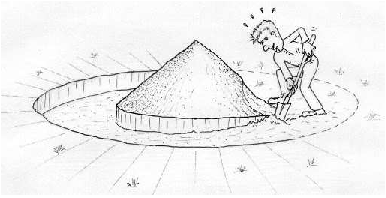
\includegraphics[scale=0.8]{RepS-50.png} 
 
  \hfill{\footnotesize \url{http://maths-msf.site2.ac-strasbourg.fr/}}
  \end{minipage}